\section{Theorie}
\label{sec:Theorie}
Unter einer Linse wird allgemein ein Objekt verstanden, welches meist optisch dichter als das es umgebende Medium ist.
Beim Übergang eines Lichtstrahls zwischen zwei Medien unterschiedlicher optischer Dichte treten nach dem Brechungsgesetz Brechungseffekte auf.
In der Optik wird zwichen verschiedenen Linsen unterschieden.
Eine Sammellinse wird zum Linsenrand hin dünner, sie bündelt parallel einfallendes Licht in dem sogennanten Brennpunkt. Entsprechend sind die Brennweite $f$ und die Bildweite $b$ positiv gezählt und es ensteht, wie in Abbildung \ref{fig:sammelli} ein reeles Bild. Mit dem Begriff reeles Bild wird
\begin{figure}
  \caption{Schematischer Strahlverlauf bei einer Sammellinse \cite{Anleitung}}
  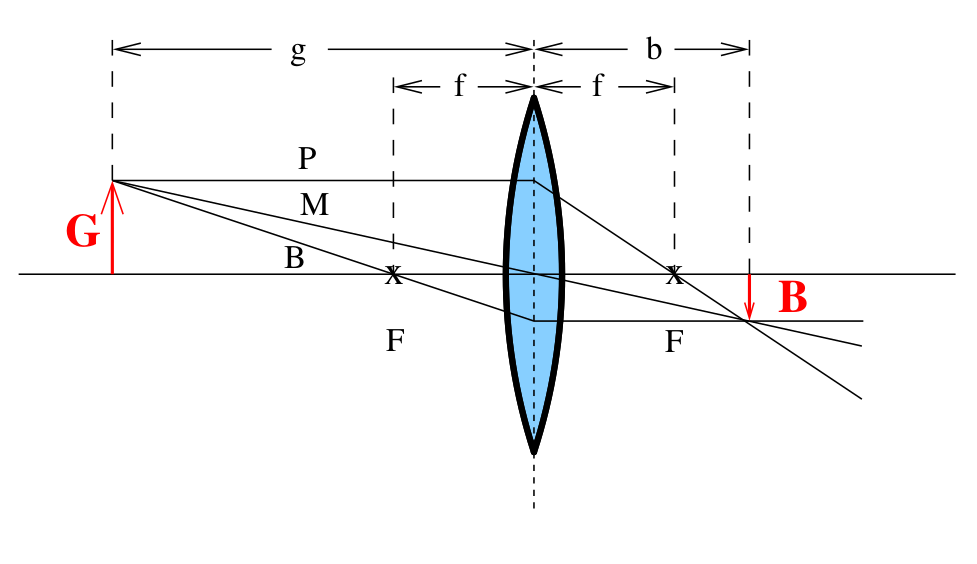
\includegraphics{Bilder/sammellinse.png}
  \label{fig:sammelli}
\end{figure}
Bei einer Streulinse
\begin{figure}
  \caption{Schematischer Strahlverlauf bei einer Streulinse \cite{Anleitung}}
  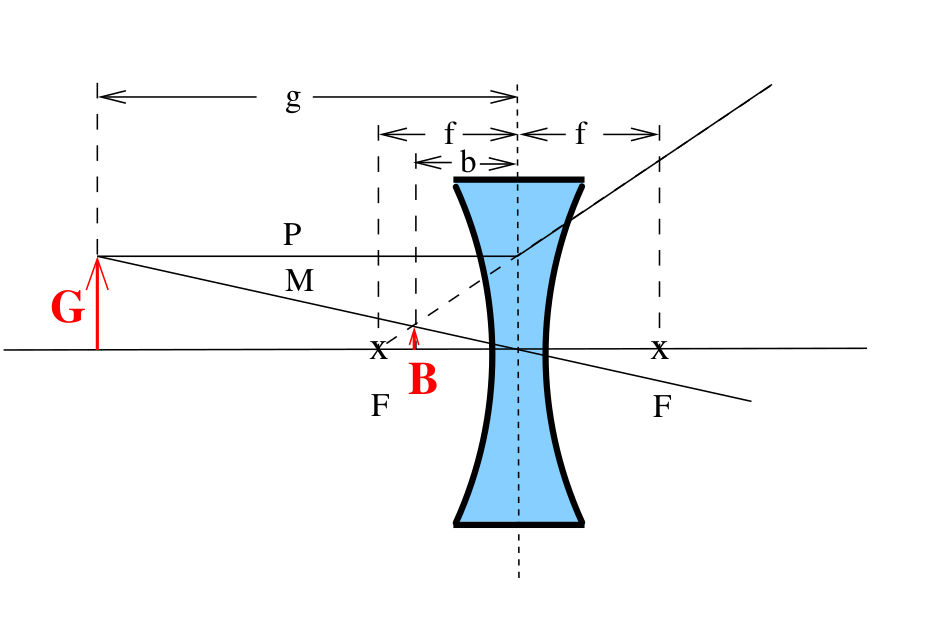
\includegraphics{Bilder/streulinse.png}
  \label{fig:streuli}
\end{figure}


\begin{figure}
  \caption{Schematischer Strahlverlauf bei einer dicken Sammellinse \cite{Anleitung}}
  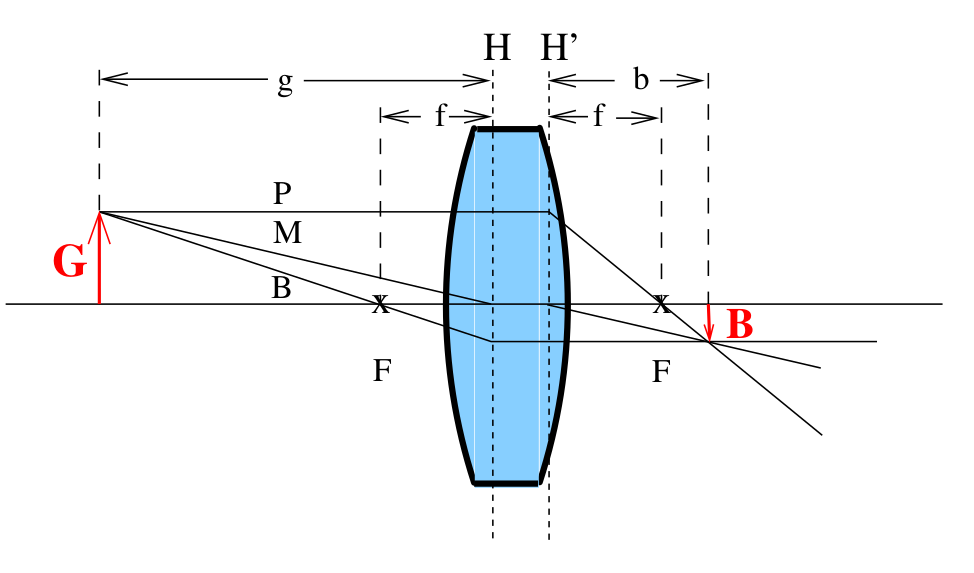
\includegraphics{Bilder/fettelinse.png}
  \label{fig:diefette}
\end{figure}


%Jaaa nice wrapfigures mal wieder!!!11
\begin{wrapfigure}[13]{r}{0.4\textwidth}
	\centering
	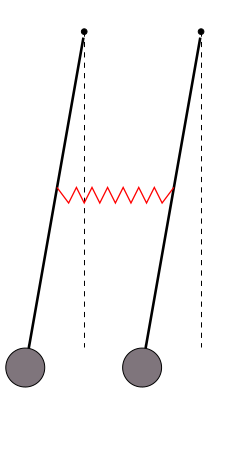
\includegraphics[width=0.4\linewidth]{Bilder/gleichphasig.png}
	\caption{Gleichsinnige Schwingung \cite{Anleitung}.}
	\label{fig:gleich}
\end{wrapfigure}
\FloatBarrier
